\section{Arabinose-induced binding of AraC protein to araI2 activates the araBAD operon promoter}

\subsection{Нормальное название}

Вызванное присутствием арабинозы связывание белков AraC и AraI активирует промотор оперона araBAD

\subsection{Абстракт}
Было обнаружено, что состояние araI в ДНК кишечной палочки, занятой белком AraC, изменяется с двух на четырехоборотную при добавлении арабинозы-индуктора.  Участок AraI можно разделить на две смежные области: AraI1 и AraI2.  aral1 связывает как связанный с лигандом, так и свободный от лиганда белок Arac, тогда как aral2  связывает белок AraC только в присутствии арабинозы.  Мутация aral и известная мутация araС привели к потере связей в aral2, в то время как связывание с araI1 не было затронуто.  Оба мутанта не смогли активировать промотор оперона araBAD.  Мы предполагаем, что занятость связей aral2 белком AraC ведет к распознаванию РНК-полимеразой промотора araBAD и что aral действует как механизм переключения, позволяющий формам белка AraC выступать и репрессором, и активатором, регулируя промотор araBAD. 

\subsubsection{Примечание}
Короче, о чем статья по факту: кишечная палочка кушает глюкозу, но если глюкозы нет, но есть арабиноза (это тоже сахар такой), то включается Арабинозный оперон araBAD, способствующий метаболизмы арабинозы. Если в среде есть глюкоза, действие оперона подавляется.
На картинке показан сам оперон araBAD: в отсутствии арабинозы димер araC контактирует с O2 и с I1, формируя петлю ДНК в 210bp.
\\
В присутствии же арабинозы (низ картинки) araC загибается, сохраняя контакт с araI1 и привязывается к соседнему araI2. Это формирует петлю ДНК и начинается транскрипция.


\subsection{Картинки}
\begin{figure}[H]
	\centering \subfigure{
		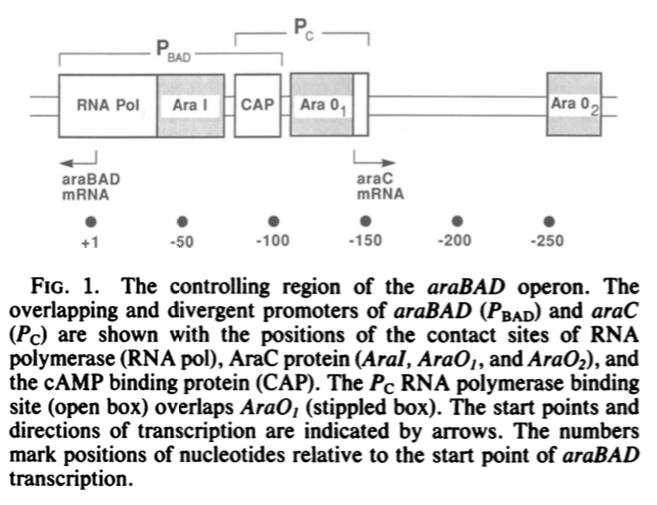
\includegraphics[width=0.35\linewidth]{a41.jpg} \label{0r} }  
	\subfigure{
		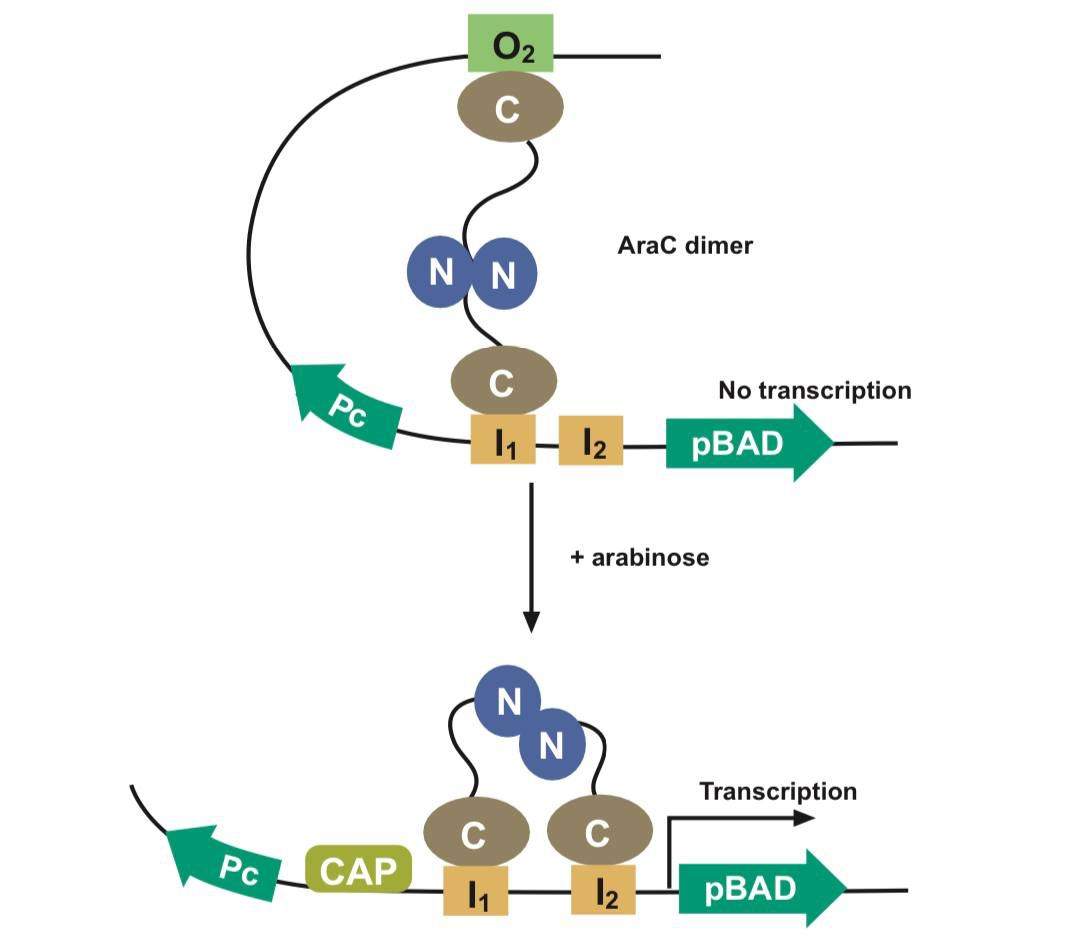
\includegraphics[width=0.35\linewidth]{a46.jpg} \label{1r} }
	\caption{Первая картинка и дополнение к ней}
\end{figure}
Здесь сама схема устройства araBAD: 
По сути, здесь то же самое, что на предыдущей картинке, только ущербно: пересекающиеся и разделенные области araBAD и araC. Начальные точки (стратуем отсюда) и направления транскрипции показаны стрелками. Числа для обозначение положений нуклеотидов  относительно начальной точки транскрипции araBAD.
\begin{figure}[H]\label{ul}
	\center{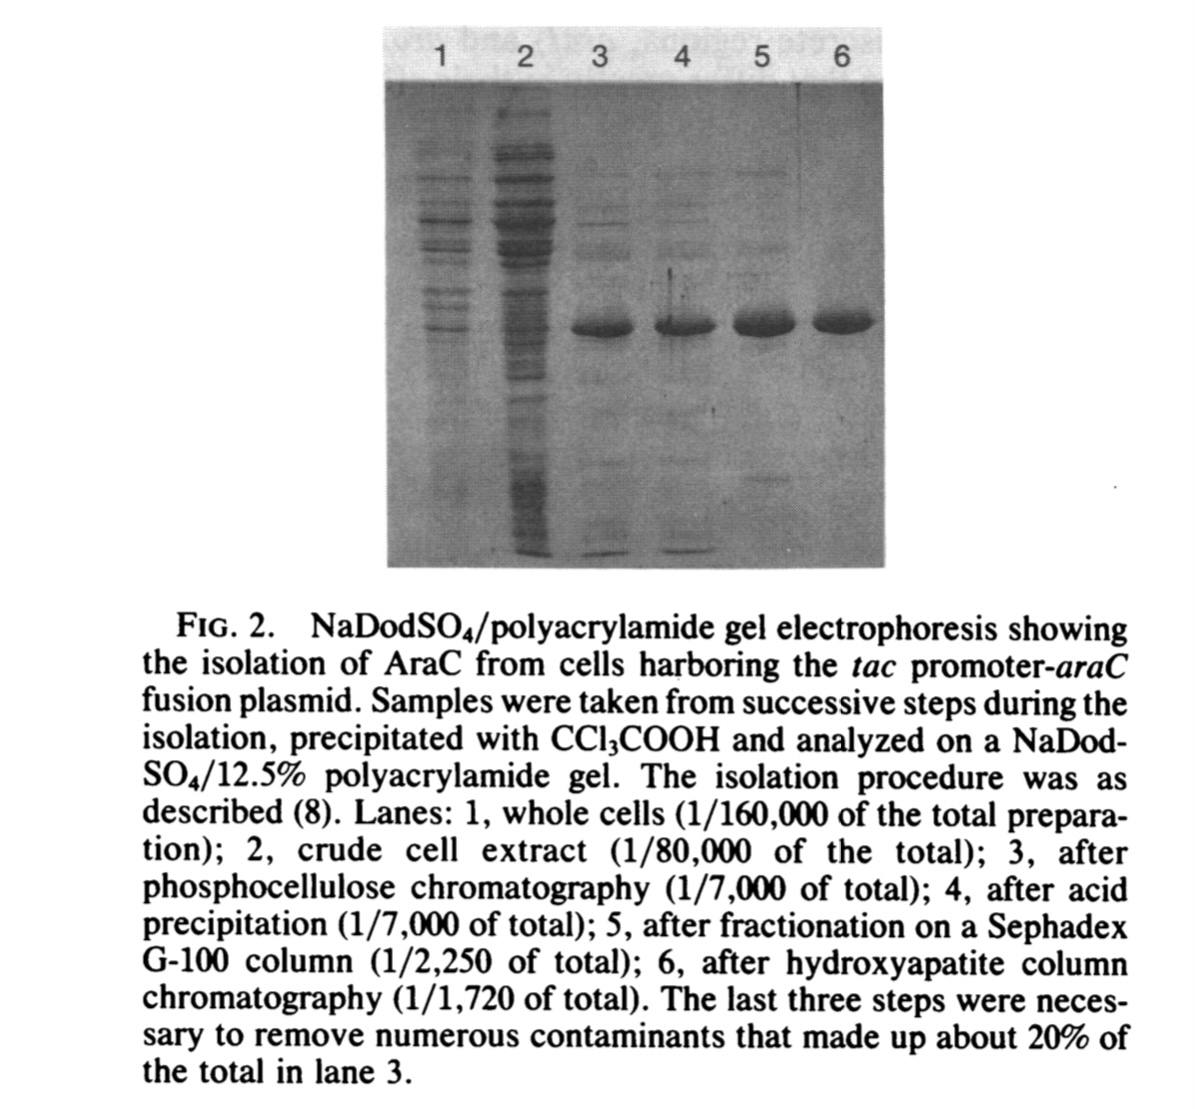
\includegraphics[scale=0.2]{a42.jpg}}
	\caption{Вторая картинка}
\end{figure} 
Электрофорез в геле, показывающий разные стадии отделения araC от клеток. Помещаем смесь разных кусков ДНК в гель, с концов прикладывает постоянный ток, и оно начинает ехать. Чем легче фрагмент, тем больше проедет.
\begin{figure}[H]\label{ul}
	\center{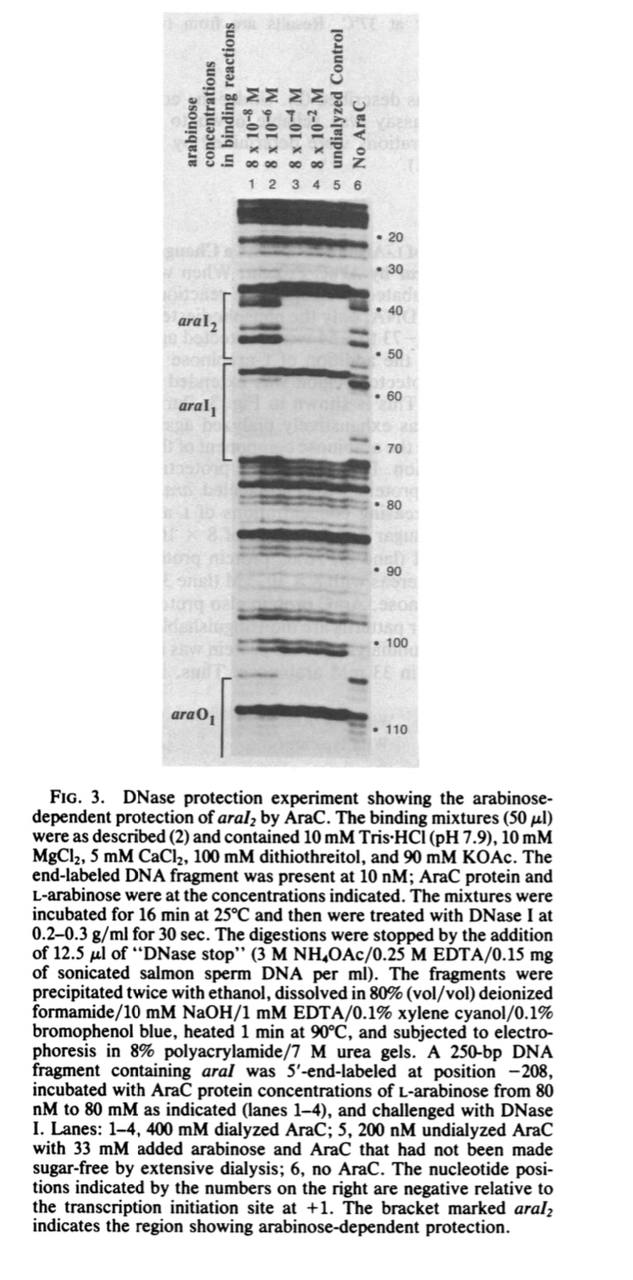
\includegraphics[scale=0.3]{a43.jpg}}
	\caption{Третья картинка}
\end{figure} 

Смотрим на зависящее от наличия арабинозы ограждение araI2 с использованием araC. Метод, который они используют, называется DNASe protection assay, он исследует взаимодействия ДНК и белков: есть молекула ДНК, есть всякие ДНКазы, которые её расщепляют в определенном месте, например, где идут буквы АТАСАС, или еще какие другие. Таких ферментов много, и каждый имеет вот такую уникальную последовательность, в которой он расщепляет ДНК. Используя разные наборы таких днказ, можно, комбинируя их, установить, где сидит белок. Скобочка с araI2 определяет изменяющуюся при наличии арабинозы область.

\begin{figure}[H]\label{ul}
	\center{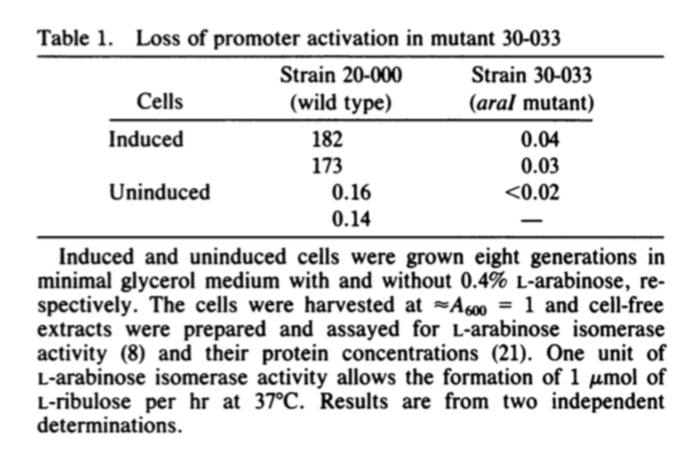
\includegraphics[scale=0.4]{t41.jpg}}
	\caption{Таблица 1}
\end{figure} 
Индуцированные и нет, обычные и мутировавшие клетки изучали на предмет активации промотора.
\begin{figure}[H]\label{ul}
	\center{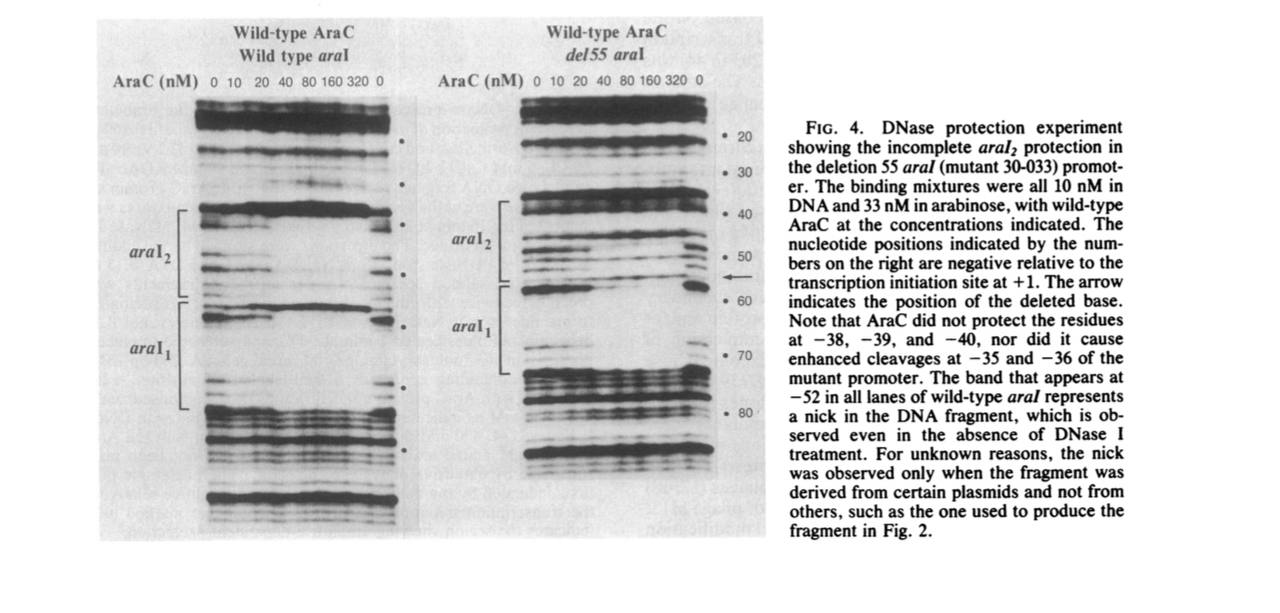
\includegraphics[scale=0.4]{a44.jpg}}
	\caption{Четвертая картинка}
\end{figure} 
Снова трюки с днказой при делеции 55 araI (мутировавшего) промотора. Стрелочкой на -52 на всех немутировавших разрыв в фрагменте ДНК.
\begin{figure}[H]\label{ul}
	\center{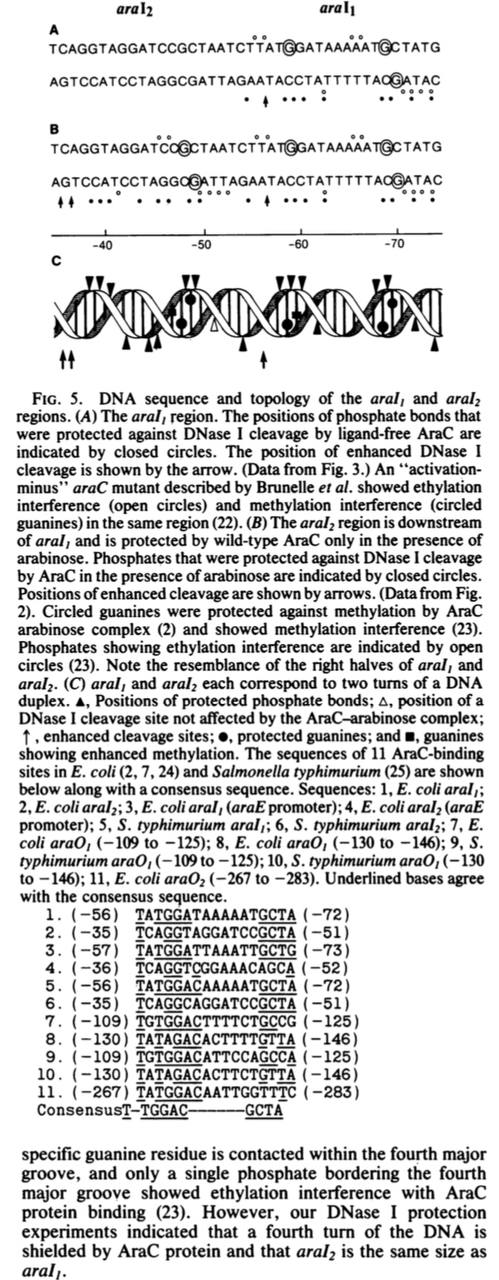
\includegraphics[scale=0.4]{a45.jpg}}
	\caption{Пятая картинка}
\end{figure}
Последовательность и топологи ДНК в областях araI1 и araI2.
Положения фосфатных связей, которые были защищены от расщепления ДНКазой безлигандным AraC, показаны темными кружками.  
В - Фосфаты, которые были защищены от расщепления ДНКазой I с помощью AraC в присутствии арабинозы, обозначены закрашенными кружками.  Позиции усиленного расщепления показаны стрелками.  Обведенные в кружки гуанины были защищены от метилирования комплексом арабинозы AraCи вмешались в метилирование. Фосфаты, показывающие нарушение этилирования, обозначены светлыми кружками. 
Обратите внимание на сходство правых половинок aral и aral, каждый соответствует двум виткам дуплекса ДНК.